\documentclass[landscape,footrule]{foils}
\usepackage[lecture-serie]{foiltex-extra}
\usepackage{crysymb}
\usepackage{graphics}
\usepackage[pdftex]{graphicx} 




\newcommand{\lecture}{Performance evaluation}
\newcommand{\lserie}{LTAT.02.004 Machine Learning II}
\newcommand{\ldate}{11 February, 2025}
\newcommand{\lauthor}{Sven Laur}
\newcommand{\linst}{University of Tartu}
\graphicspath{{./illustrations/}}
%\MyLogo{\lserie.\  Performance evaluation, \ldate}


\newcommand{\leqm}{\ \leq_m}


\newcommand{\bigvskip}{\vskip 2em}
\newcommand{\lastline}{\vspace*{-2ex}}
\newcommand{\spreadappart}{\vspace*{\fill}}
\renewcommand{\vec}[1]{\boldsymbol{#1}}

\DeclareMathOperator{\supp}{supp}
\DeclareMathOperator{\conf}{conf}
\DeclareMathOperator{\precision}{precision}
\DeclareMathOperator{\recall}{recall}


\newcommand{\fpar}[2]{\frac{\partial#1}{\partial#2}}

\begin{document}
\titlefoil

\foilhead[-0.5cm]{Can we quantify model performance at all?}

\centerline{
\includegraphics[height=4cm]{midjourney_01}\hspace*{0.5cm}
\includegraphics[height=4cm]{midjourney_02}\hspace*{0.5cm}
\includegraphics[height=4cm]{midjourney_03}\hspace*{0.5cm}
}

For some machine learning tasks there is no direct performance measure
\begin{triangles}
\item speech synthesis
\item conversational chat bots
\item image and music generation tasks
\end{triangles}
\vspace*{1cm}

For all of these tasks we can define many surrogate measures
\begin{triangles}
\item understandability and expressiveness of speech
\item grammatical correctness and adherence of other implicit patterns  
\end{triangles}   

\foilhead[-1cm]{Why do we estimate performance?}

\begin{triangles}
\item To estimate how does the algorithm perform in the future
\begin{diamonds}
\item This is the most important question in the practice 
\item We are interested on performance of a particular predictor\vspace*{2ex} 
\end{diamonds}

\item To find the best hyperparameter instance for our dataset   
\begin{diamonds}
\item It is quite tricky task if we consider all subtleties 
\item We are comparing different algorithm instances on our data\vspace*{2ex}
\end{diamonds}


\item To compare different algorithms and choose the best 
\begin{diamonds}
\item This is needed to justify the development of a new algorithm 
\item We are comparing average behaviour of algorithms\vspace*{2ex} 
\end{diamonds}

\item To see if there is a dependence between input and the output
\begin{diamonds}
\item Studies in biology or sociology are all about causal dependencies
\item We are interested in statistically significant performance levels 
\end{diamonds}

\end{triangles}


\foilhead[-1cm]{Short list of goodness measures}

Some goodness measures for classification
\begin{triangles}
\item Accuracy -- the percentage of correctly classified observations
\item Precision -- the percentage of correct labels among positive guesses 
\item Recall -- the percentage of positive cases that are detected
\end{triangles}
\vspace*{1cm}

Some goodness measures for regression
\begin{triangles}
\item Normalised mean square error
\item Normalised mean absolute error
\item Trimmed mean square and absolute error estimates  
\end{triangles}

\foilhead[-1.0cm]{Handwritten digit recognition task}

MNIST database of handwritten digits
\begin{triangles}
\item  $28\times28$ grayscale images of numbers 
\item Training set contains 60,000 images.
\item Test set contains 10,000 images.
\item We consider separation of two classes.
\end{triangles}

\vspace{1cm}
\centerline{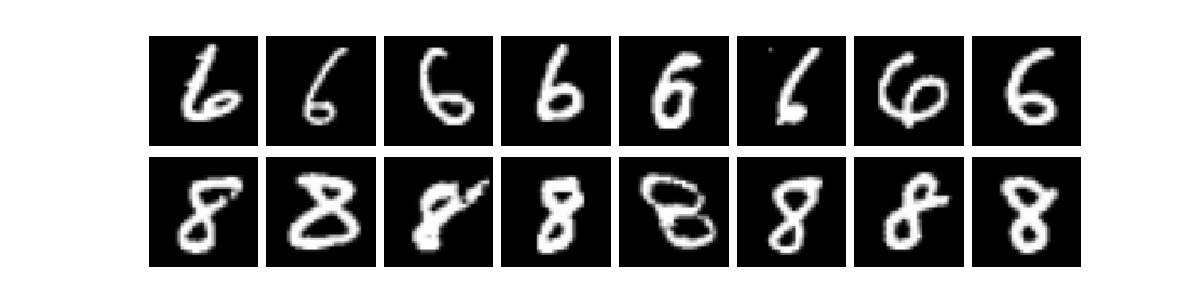
\includegraphics[height=5cm]{mnist_sample_plot}}


\foilhead[-1.0cm]{Scaling laws}

The performance of a classification algorithm depends on three factors:
\begin{triangles}
\item complexity of a model,
\item the amount of training data,
\item the amount of computational resources.
\end{triangles}

\vspace*{1cm}

There are theoretical scaling laws.
\begin{diamonds}
\item Statistical Learning Theory
\item Gives conservative relation between dataset size and performance.  
\end{diamonds}

\vspace*{1cm}

There are empirical scaling laws.
\begin{diamonds}
\item Govern  the architectural search of foundational  models.
\item Tells how much data and compute are needed to get target performance.
\end{diamonds}

\foilhead[-1.0cm]{Examples of scaling laws}

We can always fix the model and vary the compute or the dataset size.  

\vspace{1cm}
\centerline{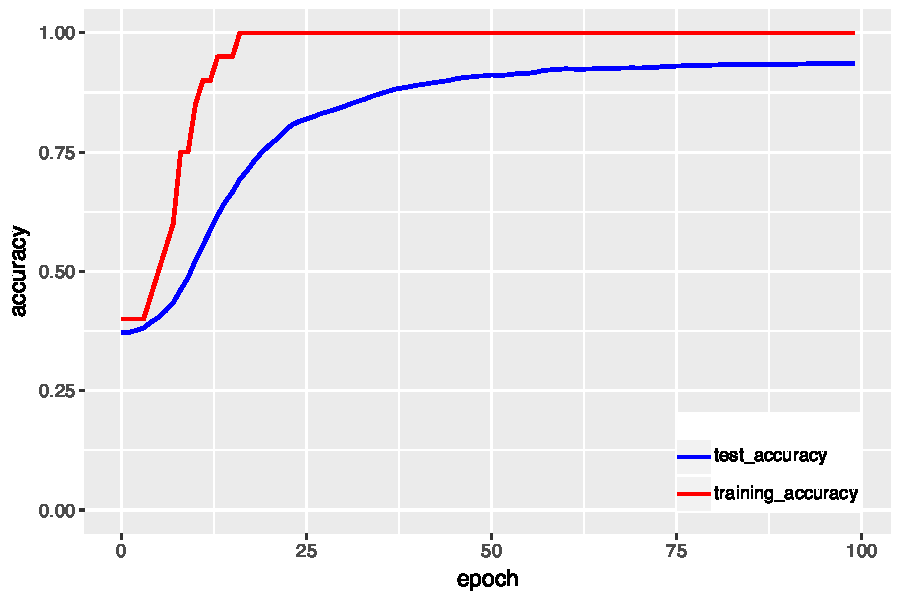
\includegraphics[height=7cm]{scaling-law-i}\hspace{1cm} 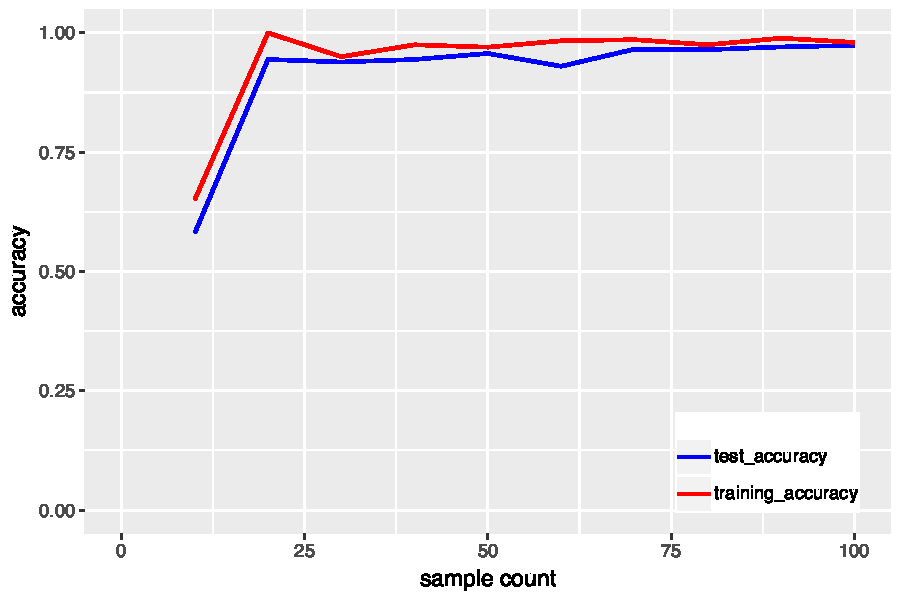
\includegraphics[height=7cm]{scaling-law-ii}}

There is always a discrepancy between test and training performance.
\begin{triangles}
\item This leaves some ambiguity about the limiting  performance.
\item Random choices are another source of ambiguity that limits utility.
\end{triangles}



\foilhead[-1.0cm]{Data-bound learning tasks}
\illustration[scale=1.1, trim = 0cm 0cm 0cm 0cm, clip]{data_bound_task}

A learning task can be hard for following reasons:
\begin{triangles}
\item data bound -- there is not enough (labelled) data
\item algorithm bound -- we do not have the right algorithm
\item compute bound -- we cannot finalise optimisation
\end{triangles}

\foilhead[-1.0cm]{What is overfitting?}

\illustration[scale=1.25, trim = 0cm 0cm 0cm 0cm, clip]{overfitting}

\begin{triangles}
\item Overfitting occurs when only the training performance decreases
\item Overfitting = difference between training and limiting performance
\item Overfitting is inevitable for stabilised models. The extent is important
\end{triangles}




%\foilhead[-1cm]{Accuracy as a function of training set size}
%\enlargethispage{1cm}
%\illustration[scale=1.2]{perceptron_vs_conv_network_performance}
%\vspace{-3ex}
%\begin{triangles}
%\item Two models were trained on the MNIST dataset of handwritten digits
%\item Both test and training error where reported for various training set sizes
%\end{triangles}


\foilhead[-1cm]{Models with distinct performance}
\enlargethispage{1cm}
\illustration[scale=1.2]{perceptron_vs_conv_network_performanceover_folds}
\vspace{-3ex}
\begin{triangles}
\item The MNIST test set consits of 10000 samples 
\item Accuracy for reduced test sets consisting of 1000 samples
\end{triangles}

%\foilhead[-1cm]{Accuracy depends on the training set}

%\enlargethispage{1cm}
%\illustration[scale=1.2]{perceptron_vs_conv_network_stability_match}
%\vspace{2ex}
%\begin{triangles}
%\item We trained two models on independently sampled training sets
%\item We measured the fraction of coinciding lables on the fixed test set
%\end{triangles}

\foilhead[-0.0cm]{How much samples are needed?}

\illustration[scale=0.65, trim = 0cm 0cm 0cm 0cm, clip]{sample_size_vs_precision}

\begin{triangles}
\item 9600 samples are needed to estimate accuracy with precision $1\%$
\item If true accuracy $\geq$ 90\% then the number of samples drops to 3500
\item Performance increments of size $0.1-0.5\%$ are relevant in practice
\item This means test sets with sizes around $35,000-960,000$ 
\end{triangles}


\foilhead[-0.5cm]{Absolute vs relative performance}

\illustration[scale=1.0, trim = 0cm 0.3cm 0cm 0cm, clip]{relative_accuracy}

Relative difference in accuracy can be measured more precisely.
\begin{triangles}
\item Make predictions $\hat{\vec{y}}_A$ and $\hat{\vec{y}}_B$ on unlabelled data.
\item Find data points on which predictions differ $\mathcal{D}=\set{i: \hat{\vec{y}}_A[i]\neq \hat{\vec{y}}_B[i]}$.
\item Estimate relative difference in accuracies $\Delta_\mathcal{D}$ on the set of differences $\mathcal{D}$.
\item Estimate the relative size $p_\mathcal{D}$ of $\mathcal{D}$ and rescale the difference:
\begin{align*}
\mathsf{accuracy}_A-\mathsf{accuracy}_B= p_\mathcal{D}\cdot \Delta_\mathcal{D}\enspace.
\end{align*}  
\end{triangles}

\foilhead[-0.5cm]{Shortcuts for relative performance}

\illustration[scale=1.0, trim = 0cm 0.3cm 0cm 0cm, clip]{relative_accuracy}

The alternative formula $p_\mathcal{D}\cdot \Delta_\mathcal{D}$ is more approachable
\begin{triangles}
\item The proportion $p_\mathcal{D}$ can be computed without knowing true labels
\item $\Delta_\mathcal{D}$ can be estimated by labelling 1000 random samples form $\mathcal{D}$
\end{triangles}
\vspace*{1cm}

We can bound the relative difference without knowing true labels:
\begin{align*}
\abs{\mathsf{accuracy}_A-\mathsf{accuracy}_B}\leq p
\end{align*}

\foilhead[-1.0cm]{Near ideal precision-recall graph}

\centerline{\includegraphics[height=8cm]{precision_recall_1}\hspace{0cm} \includegraphics[height=9.5cm]{pr_lable_separation_1}}

\foilhead[-1.0cm]{Quick dropp-offs in precision-recall graph}

\centerline{\includegraphics[height=8cm]{precision_recall_2}\hspace{0cm} \includegraphics[height=9.5cm]{pr_lable_separation_2}}

\begin{triangles}
\item  There must be a batch of negative data points with high scores.
\item  The score stabilises when the ratio of positives and negatives stabilises.
\end{triangles}


\foilhead[-1.0cm]{Which model is better?}
\illustration[scale=1.0, angle=0, trim = 0cm 0cm 0cm 0cm, clip]{accuracy_challenge}

\begin{triangles}
\item Method A outputs the correct label in 75\% cases on average
\item Method B outputs the correct lable in 85\% cases on average
\item Which method works significantly better on future data? 
\end{triangles} 

\foilhead[-1.0cm]{How to model future?}

\illustration[scale=0.9, angle=0, trim = 0cm 0cm 0cm 0cm, clip]{future_modelling}


\foilhead[-0.0cm]{Future holds only 100 prediction tasks}

\illustration[scale=0.7, trim = 0cm 0cm 0cm 0cm, clip]{accuracy_challenge_100}

Both methods are roughly equal although the accuracies are very different. 

\foilhead[-0.0cm]{Future holds 10000 prediction tasks}

\illustration[scale=0.7, trim = 0cm 0cm 0cm 0cm, clip]{accuracy_challenge_10000}

The method B is clearly superior to the method A as expected. 

\foilhead[-1.0cm]{Direct consequences}

\begin{triangles}
\item The performance of a method fluctuates over all possible futures
\item The magnitude of fluctuations decreases with the sample size
\item True performance is defined as a limit over the infinite sample
\item A finite estimate will always fluctuate around the true performance
\end{triangles}
\vspace*{1.5cm}

Finite number of new observations in the future means that
\begin{triangles}
\item certain performance differences are irrelevant
\item the pursuit of optimal performance is pointless
\end{triangles}

\vspace*{2.0cm}
\textbf{Simplifying assumption}
\begin{triangles}
\item We assume that the number of new observations is unbounded.
\end{triangles}








%\foilhead[-1cm]{Different methods vs typical learning tasks}
%\enlargethispage{1cm}
%\illustration[scale=0.8]{convergence-small}
%\vspace*{-0.0cm}
%$\triangleright$  Depends on data and a target function\\
%$\triangleright$  Depends on the size of training data and method itself



\foilhead[-1cm]{How to estimate performance in the future}
\enlargethispage{1cm}
\illustration[scale=0.8]{expected-goodness}

For any prediction algorithm we can find its expected goodness in the future.

\textbf{Practice.} Average goodness over a long enough series of future samples.

\begin{triangles}
\item Sampling should not change the data source in the future. 
\item All future samples should be independent from each other. 
\end{triangles} 
\vspace*{2ex}

\textbf{Theory.} We should find expected goodness over the data distribution.
\begin{triangles}
\item The distribution always exists although we might not know it.  
\item Expected value exists even if the number of future samples is limited.
\end{triangles} 
\bigskip



\foilhead[-1cm]{Are these assumptions satisfied in practice?}

\textbf{Assumption I.} Data distribution does not change
\begin{triangles}
\item Some changes in data can be modelled
\item If radical changes occur the model must be retrained
\item Sometimes predictions must be valid regardless of inputs  \vspace*{1cm}
\end{triangles}

\textbf{Assumption II.} Future samples are independent from each other
\begin{triangles}
\item This assumption is always violated in text analysis
\item This assumption is always violated in time-series analysis
\item Correlation between future samples creates overconfidence
\item This effect can be corrected with more careful sampling of a test set
\end{triangles}

\foilhead[-1cm]{Notation and terminology}

\textbf{Spaces}
\begin{triangles}
\item $\DDD$ -- data distribution
\item $\XXX$ -- input space, feature space
\item $\YYY$ -- output space, target space
\item $\FFF\subseteq\set{f:\XXX\times\Omega\to\YYY}$ -- model class\vspace*{0.5cm}
\end{triangles}

\textbf{Instances}
\begin{triangles}
\item $\vec{x}\in\XXX$ -- instance
\item $y$ -- true value of an instance, target value
\item $\hat{y}=f(\vec{x})$ -- predicted target value\vspace*{0.5cm}
\end{triangles}

\textbf{Loss:}
\begin{triangles}
\item $L:\YYY\times\YYY\to\RRR$ --  the cost of using prediction $\hat{y}$ instead of $y$
\end{triangles}
 

 
\foilhead[-1cm]{Theoretical formulation}

Let $\DDD$ be the distribution of $(x,y)$ pairs where $x$ is the input and $y$ is the target of a prediction algorithm $f$. 
\bigskip

Let $L:\YYY\times\YYY\to\RR$ be the \emph{loss function} which takes in the predicted value $\hat{y}$ and the actual value $y$ and outputs resulting loss.
\bigskip

Then the corresponding \emph{risk} $R(f)$ is computed as \emph{mathematical expectation}
\begin{align*}
 R(f):=\EXP_\DDD(L(f(x), y))=\int\limits_{(x,y)\in\DDD} L(f(x), y) dF(x,y)
\end{align*}   
where $F$ is the corresponding probability measure.

\foilhead[-1cm]{Practical example}

\begin{triangles}
\item Let $f(x_1,x_2)\equiv 0$ and let $L(\hat{y}, y)= (y-\hat{y})^2$. What is the risk $R(f)$ if the next data sample is chosen uniformly from the following table.
\bigskip

\begin{center}
\begin{tabular}{|c|c|c|}
\hline
$x_1$ & $x_2$ & $y$\\ 
\hline
0 & 0 & 0\\
0 & 0 & 1\\
0 & 1 & 1\\
1 & 0 & 0\\
1 & 1 & 1\\
0 & 0 & 0\\
\hline
\end{tabular}
\bigskip

\end{center}
\item Propose a new prediction rule $f_*$ that minimises the risk. 
\item Is there always a prediction rule that minimises the risk?
\end{triangles}

\foilhead[-1cm]{Empirical risk estimation}

When the sample $D_N=\set{(\vec{x}_1,y_1),(\vec{x}_2,y_2),\ldots, (\vec{x}_N, y_N)}$ is \emph{representative} then we can approximate risk $R(f)$ with \emph{empirical risk}:
\begin{align*}
  R_N(f)=\frac{1}{N}\cdot\sum_{i=1}^N L(f(\vec{x}_i), y_i)\enspace.
\end{align*} 
\hspace*{1cm}

\textbf{IID sampling assumption.} The following conditions assure that the sample data $D_N$ is representative (with high probability).
\begin{triangles}
\item All samples are independent from each other. 
\item All samples are drawn from the same distribution.
\item Future samples come from the same distribution as the data $D_N$.
\end{triangles}

\foilhead[-1cm]{Empirical risk}
\enlargethispage{1cm}
\centerline{
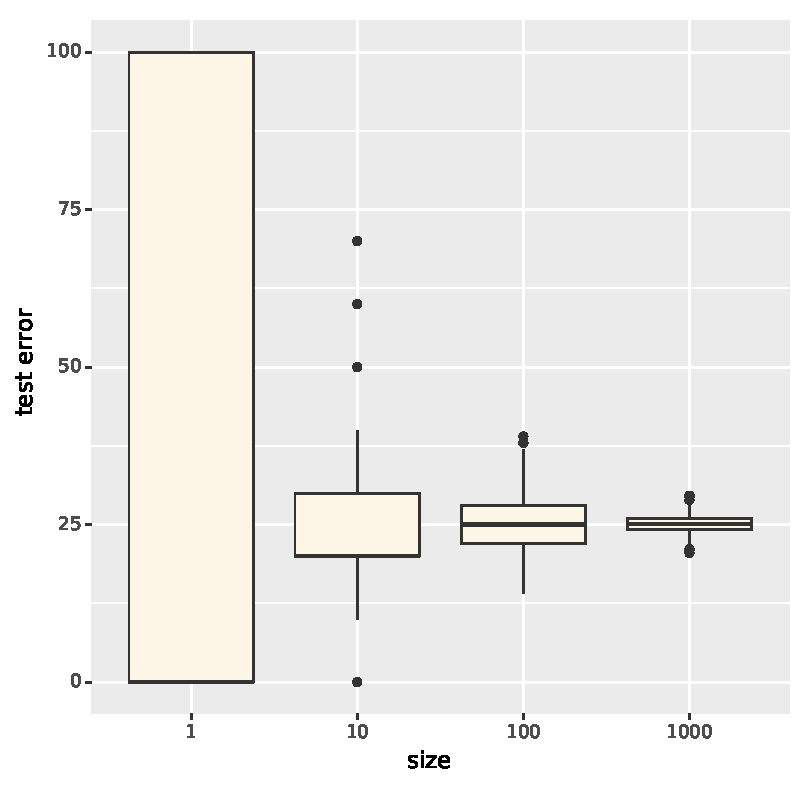
\includegraphics[scale=0.8]{test_error_fluctuations_1}\hspace*{0.5cm}
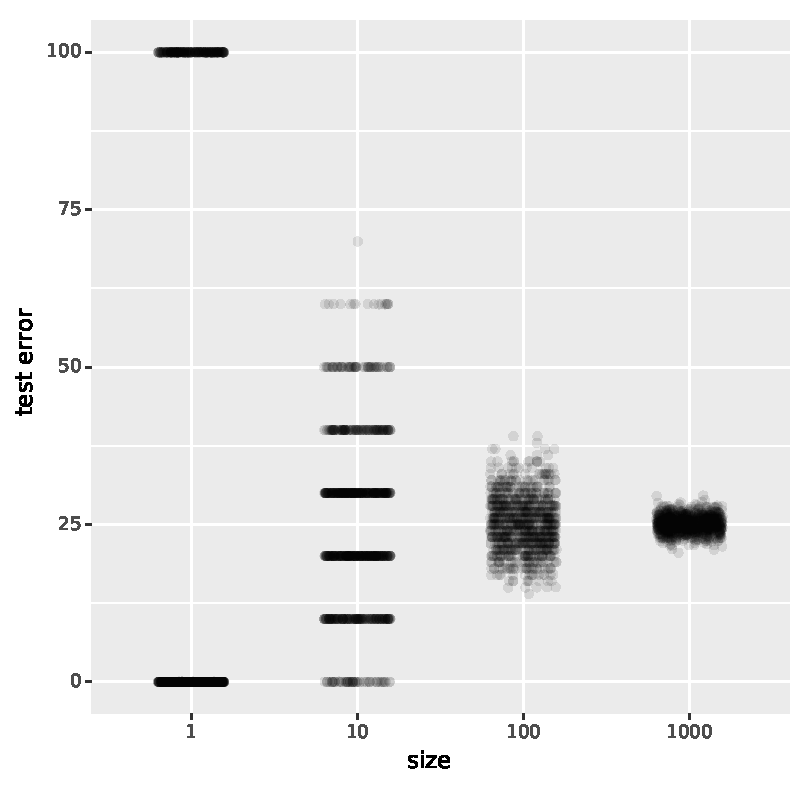
\includegraphics[scale=0.8]{test_error_fluctuations_2}}

\vspace*{-0.0cm}
$\triangleright$  depends on the dataset\\
$\triangleright$  statistical fluctuations decrease with size



\foilhead[-1cm]{Law of large numbers}

\textbf{Central limit theorem.}
Let $z_1, \ldots, z_N$ be independent and identically distributed samples form a \emph{real-valued distribution} with a \emph{finite standard deviation} $\sigma$ and \emph{mean} $\mu$. Then the random variable 
\begin{align*}
S=\sqrt{N}\Biggl(\frac{1}{N}\cdot \sum_{i=1}^N z_i -\mu\Biggr)
\end{align*}
converges \emph{in distribution} to normal distribution $\NNN(mean=0, sd=\sigma)$.  

\foilhead[-1cm]{Translation}


Under mild assumptions the empirical risk $R_N(f)$ converges to risk $R(f)$ and we can actually use normal distribution to estimate probabilities:
\begin{align*}
\pr{\abs{R_N(f)-R(f)}\geq \varepsilon} \lesssim 2\cdot \int\limits_{-\infty}^\varepsilon\frac{\sqrt{N}}{\sqrt{2\pi}\sigma}\exp{-\frac{N t^2}{2 \sigma^2}}dt
\end{align*}
for a finite value $\sigma$ where $\sigma^2$ is the variance of loss $\VAR(R(f))$.
\vspace*{1cm}

\textbf{Reasoning}
\begin{triangles}
\item If $(\vec{x}_i, y_i)$ are IID samples then $z_i=L(f(\vec{x}_i), y_i)$ are also IID samples.
\item By definition $\mu=\EXP(z)=\EXP(L(f(\vec{x}),y))=R(f)$.
\item CLT assumes that risk $\mu$ is finite and standard deviation $\sigma$ is finite.
\end{triangles}
\bigskip


\foilhead[-1cm]{Visual representation}

\illustration[scale=0.8]{normal_approximation}

\vspace*{-0.5cm}

Convergence implies that the centre area of is well approximated 
\begin{triangles}
\item 90\% confidence intervals are roughly the same for both distributions
\end{triangles}

\end{document}

